%% SECTION HEADER /////////////////////////////////////////////////////////////////////////////////////
\section{The \acs{madif} under variable temperature conditions}
\label{sec:madifTemp}

%% SECTION CONTENT ////////////////////////////////////////////////////////////////////////////////////
In addition to the referenced \ac{madif} obtained for +20\unit{\degreeCelsius}, a study of wave propagation at temperatures T=\(\left[-10,\,0,\,+10,\,+30,\,+40,\,+50\right]\)\unit{\degreeCelsius} was carried out.
To determined temperature-dependent simulations of \ac{gw} propagation in \ac{hsc}, the material properties of the components were determined according to the methodology described in section~\ref{sec:temp}.

The temperature effect on the \acp{madif} is developed based on the \ac{fcgm} and removed core cells as a damage model.
The analysis used both \acp{di}, i.e. the \ac{rmsd} and the \ac{cc}, for the 100 \unit{\kHz} full-length signal.
The signal obtained for a healthy sample at each temperature was taken as the reference signal for each case.
\begin{table}[!tbh]
	\small
	\tabcolsep=0.25cm
	\centering
	\caption{\label{tab:fit_F_err_temp} The time-dependent coefficients and errors of the function from Eq.~(\ref{eq:function_1}) fitted to \acp{di} based on the \acf{fcgm} - core.}
\begin{tabular}{c|cc|cc}
	\toprule \multirow{3}{*}{T \unit{\degreeCelsius}} & \multicolumn{2}{c|}{\ac{rmsd}} & \multicolumn{2}{c}{\ac{cc}}\\
	&\multicolumn{2}{c|}{100 \unit{\kHz}}&\multicolumn{2}{c}{100 \unit{\kHz}}\\
	& \(a_i\) &  \(\delta^{\mathrm{fit}}\) \% & \(a_i\) & \(\delta^{\mathrm{fit}}\) \%\\
	\midrule
	 \multirow{3}{*}{0} & 24.72 & \multirow{3}{*}{\textcolor{green}{1.43}}& 123.8 & \multirow{3}{*}{\textcolor{green}{0.48}}\\
	 & 90.62 & & 404.2 &\\
	 & 0.57 & & 0.67 &\\
	\midrule
	\multirow{3}{*}{+10} & 6.37 & \multirow{3}{*}{\textcolor{green}{1.31}}& 42.81 & \multirow{3}{*}{\textcolor{green}{0.43}}\\
	& 24.91 & & 208.3 &\\
	& 0.67 & & 0.78 &\\
	\midrule
	\multirow{3}{*}{+30} & 3.62 & \multirow{3}{*}{\textcolor{green}{1.32}}& 3.10 & \multirow{3}{*}{\textcolor{green}{0.42}}\\
	& 17.38 & & 41.95 &\\
	& 0.71 & & 0.92 &\\
	\midrule
	\multirow{3}{*}{+40} & 2.43 & \multirow{3}{*}{\textcolor{green}{1.38}}& 0.95 & \multirow{3}{*}{\textcolor{green}{0.44}}\\
	& 19.76 & & 22.09 &\\
	& 0.72 & & 0.94 &\\
	\bottomrule
\end{tabular}
\end{table}

The temperature-dependent \acp{madif} based on \ac{rmsd} and \ac{cc} are presented in Fig.\ref{fig:madif_temp_rmsd} and Fig.~\ref{fig:madif_temp_cc}, respectively.
It is observed that the variation in ambient temperature condition can substantially influence the \ac{madif} values.
From Fig.~\ref{fig:madif_temp_rmsd}, it can be seen that the errors increase the higher the absolute difference between ambient and reference temperature.
Therefore, the assumed linear model of the temperature-dependent material properties of the components used in the simulation is not sufficiently accurate with the real object.
It is particularly evident for temperatures of 0\unit{\degreeCelsius} and -10\unit{\degreeCelsius}, where the \ac{madif} for damage size more than 25 \unit{\mm} does not reach the values obtained experimentally.
The best results were achieved for a temperature of +10\unit{\degreeCelsius}, for which the absolute error does not exceed 2 mm over the full range of damage sizes. 
\begin{figure}[!tbh]
	\begin{center}
		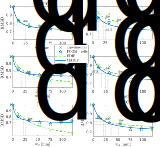
\includegraphics[width=0.95\textwidth]{Chapter_8/MADIF_temp_RMSD}
	\end{center}
	\caption{The \acf{madif} and the \acf{edif} based on the \acf{rmsd} 100 \unit{\kHz}.}
	\label{fig:madif_temp_rmsd}
\end{figure}
\begin{figure}
	\begin{center}
		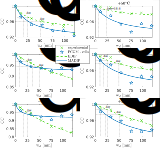
\includegraphics[width=0.95\textwidth]{Chapter_8/MADIF_temp_CC}
	\end{center}
	\caption{The \acf{madif} and the \acf{edif} based on the \acf{cc} 100 \unit{\kHz}.}
	\label{fig:madif_temp_cc}
\end{figure}